\section{Introduction}

\subsection{Overview of CGRA and SNN Inference}
Spiking Neural Networks (SNNs) represent the third generation of neural computation \cite{maass1997networks}, providing energy-efficient execution through event-driven mechanisms. However, deploying SNNs on traditional hardware (CPUs/GPUs) is inefficient due to sparse, irregular connectivity. SNNs operate on discrete spike events, causing SIMD utilization to drop sharply in von Neumann processors.

\begin{figure}[H]
    \centering
    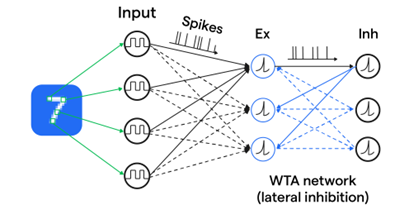
\includegraphics[width=0.8\textwidth]{images/Spiking Neural Networks (SNNs).png}
    \caption{Biological vs. Artificial Spiking Neuron Models}
    \label{fig:snn_overview}
\end{figure}

{\sloppy
To address these limitations, the proposed CGRA employs a spatially programmable 4$\times$4 mesh of Processing Elements (PEs). Each tile combines a fixed-point Multiply\-Accumulate (MAC) unit with a hardware\-implemented Leaky Integrate\-and\-Fire (LIF) neuron update engine. This unified execution model allows the array to compute sparse matrix--vector (matvec) operations and neuron dynamics in a tightly coupled, dataflow-driven manner.
}

\subsection{System Context and Execution Flow}
The CGRA is designed as a tightly integrated hardware accelerator under full control of the dual-core ARM Cortex-A9 processing system. The typical execution flow consists of:
\begin{enumerate}
    \item \textbf{Configuration Stage:} The host processor writes bitstream (context words) into the CGRA configuration memory via the CSR interface. These bitstream encode the spatial and temporal behavior of the 4×4 PE mesh.
    \item \textbf{Data Preparation:} SNN weight matrices are stored in Compressed Sparse Column (CSC) format in DDR memory. Input spike vectors and neuron states are prepared and aligned for DMA-based transfer.
    \item \textbf{Execution Phase:} The CGRA performs sparse matvec operations and LIF neuron updates in each PE according to the dynamical equation: $v[t+1] = \beta \cdot v[t] + I[t] - \lambda$.
    \item \textbf{Result Collection:} Updated membrane potentials and spike outputs are written back to DDR for use by the next simulation timestep or software post-processing.
\end{enumerate}

\subsection{Target Workload and Problem Scope}
The CGRA accelerator is optimized for sparse SNN layer updates, specifically weight matrices $W \in \mathbb{R}^{128 \times 128}$ stored in CSC format. This representation allows the accelerator to process only active presynaptic spikes by scanning the corresponding nonzero column entries, thus avoiding dense computation. 
The primary bottlenecks addressed are:
\begin{itemize}
    \item \textbf{Routing Congestion:} fan-out dominant distributions causing "Routing Black Holes."
    \item \textbf{Data Starvation:} irregular memory access patterns leading to PE idle cycles.
    \item \textbf{Precision Inefficiency:} inefficient use of bit-width in standard generic ALUs, requiring specialized 40-bit saturating logic for high-fidelity LIF updates.
\end{itemize}

The system architecture and DMA engine are designed according to the AMBA AXI Standard \cite{arm_amba_axi}, ensuring interoperability with the Zynq-7000 processing system \cite{xilinx_ug1085}.
